\documentclass[tikz,border=10pt]{standalone}
\usepackage{times}
\usepackage{amsmath,amssymb}
\usetikzlibrary{arrows.meta}

\begin{document}
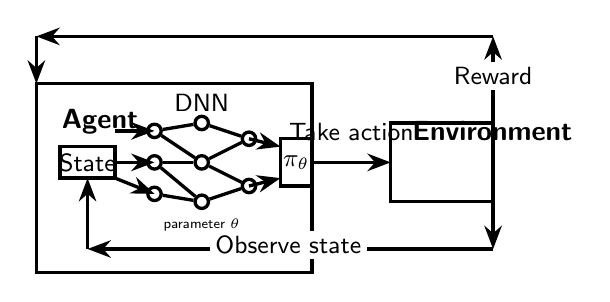
\begin{tikzpicture}[
    arrow/.style={->, >=Stealth, very thick, color=black},
    label/.style={font=\sffamily\small}
]

% ============================================================
% AGENT BOX
% ============================================================
\draw[very thick] (-0.3,0.2) rectangle (3.2,-2.2);
\node[font=\sffamily\bfseries, anchor=north west] at (-0.1, 0) {Agent};

% STATE BOX (left inside agent)
\draw[very thick] (0, -0.6) rectangle (0.7, -1);
\node[font=\sffamily\small, anchor=center] at (0.35, -0.8) {State};

% DNN VISUALIZATION (center inside agent)
% Input layer
\node[circle, draw=black, very thick, inner sep=0.06cm, fill=white] (in1) at (1.2, -0.4) {};
\node[circle, draw=black, very thick, inner sep=0.06cm, fill=white] (in2) at (1.2, -0.8) {};
\node[circle, draw=black, very thick, inner sep=0.06cm, fill=white] (in3) at (1.2, -1.2) {};

% Hidden layer
\node[circle, draw=black, very thick, inner sep=0.06cm, fill=white] (h1) at (1.8, -0.3) {};
\node[circle, draw=black, very thick, inner sep=0.06cm, fill=white] (h2) at (1.8, -0.8) {};
\node[circle, draw=black, very thick, inner sep=0.06cm, fill=white] (h3) at (1.8, -1.3) {};

% Output layer
\node[circle, draw=black, very thick, inner sep=0.06cm, fill=white] (out1) at (2.4, -0.5) {};
\node[circle, draw=black, very thick, inner sep=0.06cm, fill=white] (out2) at (2.4, -1.1) {};

% DNN connections
\draw[very thick] (in1) -- (h1);
\draw[very thick] (in1) -- (h2);
\draw[very thick] (in2) -- (h2);
\draw[very thick] (in2) -- (h3);
\draw[very thick] (in3) -- (h3);
\draw[very thick] (h1) -- (out1);
\draw[very thick] (h2) -- (out1);
\draw[very thick] (h2) -- (out2);
\draw[very thick] (h3) -- (out2);

% DNN label
\node[font=\sffamily\small] at (1.8, -0.05) {DNN};

% Parameter label
\node[font=\sffamily\tiny] at (1.8, -1.6) {parameter $\theta$};

% POLICY BOX (square, right side of agent)
\draw[very thick] (2.8, -0.5) rectangle (3.2, -1.1);
\node[font=\sffamily\small, anchor=center] at (3, -0.8) {$\pi_\theta$};

% ============================================================
% CONNECTIONS INSIDE AGENT
% ============================================================

% State to DNN input
\draw[arrow] (0.7, -0.4) -- (1.2, -0.4);
\draw[arrow] (0.7, -0.8) -- (1.2, -0.8);
\draw[arrow] (0.7, -1.0) -- (1.2, -1.2);

% DNN output to Policy
\draw[arrow] (2.4, -0.5) -- (2.8, -0.6);
\draw[arrow] (2.4, -1.1) -- (2.8, -1.0);

% ============================================================
% ENVIRONMENT BOX (smaller)
% ============================================================
\draw[very thick] (4.2, -0.3) rectangle (5.5, -1.3);
\node[font=\sffamily\bfseries, anchor=north west] at (4.35, -0.15) {Environment};

% ============================================================
% MAIN CONNECTIONS TO ENVIRONMENT
% ============================================================

% Policy to Environment (Take action)
\draw[arrow] (3.2, -0.8) -- (4.2, -0.8);
\node[label, anchor=south] at (3.7, -0.65) {Take action};

% ============================================================
% REWARD PATH (top, rectangular)
% ============================================================
\draw[arrow] (5.5, -0.3) -- (5.5, 0.8);
\draw[arrow] (5.5, 0.8) -- (-0.3, 0.8);
\draw[arrow] (-0.3, 0.8) -- (-0.3, 0.2);

\node[label, anchor=center, fill=white, inner sep=2pt] at (5.5, 0.3) {Reward};

% ============================================================
% OBSERVE STATE PATH (bottom, rectangular)
% ============================================================
\draw[arrow] (5.5, -1.3) -- (5.5, -1.9);
\draw[arrow] (5.5, -1.9) -- (0.35, -1.9);
\draw[arrow] (0.35, -1.9) -- (0.35, -1.0);

\node[label, anchor=center, fill=white, inner sep=2pt] at (2.9, -1.85) {Observe state};

\end{tikzpicture}
\end{document}
